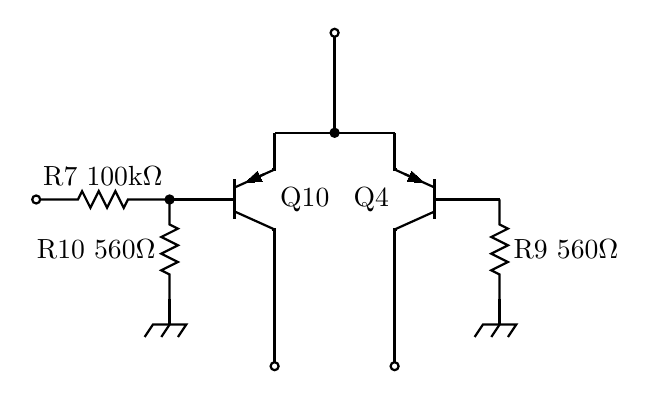
\begin{tikzpicture}[scale=2.54]
% dpic version 2014.Jan.01 option -g for TikZ and PGF 1.01
\ifx\dpiclw\undefined\newdimen\dpiclw\fi
\global\def\dpicdraw{\draw[line width=\dpiclw]}
\global\def\dpicstop{;}
\dpiclw=0.8bp
\dpiclw=0.8bp
\dpicdraw[fill=black](0,0) circle (0.007874in)\dpicstop
\dpicdraw (0,0)
 --(-0.3,0)\dpicstop
\dpicdraw (-0.3,0)
 --(-0.3,-0.1835)
 --(-0.31107,-0.1835)\dpicstop
\dpicdraw (-0.3,-0.667)
 --(-0.3,-0.4835)
 --(-0.31107,-0.4835)\dpicstop
\dpicdraw (-0.5,-0.2335)
 --(-0.5,-0.4335)\dpicstop
\dpicdraw (-0.625,-0.3335)
 --(-0.5,-0.3335)\dpicstop
\dpicdraw (-0.3,-0.1835)
 --(-0.5,-0.2735)\dpicstop
\dpicdraw (-0.35,-0.206)
 --(-0.374007,-0.216803)\dpicstop
\filldraw[line width=0bp](-0.385406,-0.191472)
 --(-0.45,-0.251)
 --(-0.362608,-0.242134) --cycle
\dpicstop
\dpicdraw (-0.3,-0.4835)
 --(-0.5,-0.3935)\dpicstop
\draw (-0.3,-0.3335) node[right=-1.5bp]{$ \textrm{Q10}$};
\dpicdraw (0,0)
 --(0.3,0)\dpicstop
\dpicdraw (0.3,0)
 --(0.3,-0.1835)
 --(0.31107,-0.1835)\dpicstop
\dpicdraw (0.3,-0.667)
 --(0.3,-0.4835)
 --(0.31107,-0.4835)\dpicstop
\dpicdraw (0.5,-0.2335)
 --(0.5,-0.4335)\dpicstop
\dpicdraw (0.625,-0.3335)
 --(0.5,-0.3335)\dpicstop
\dpicdraw (0.3,-0.1835)
 --(0.5,-0.2735)\dpicstop
\dpicdraw (0.35,-0.206)
 --(0.374007,-0.216803)\dpicstop
\filldraw[line width=0bp](0.362608,-0.242134)
 --(0.45,-0.251)
 --(0.385406,-0.191472) --cycle
\dpicstop
\dpicdraw (0.3,-0.4835)
 --(0.5,-0.3935)\dpicstop
\draw (0.3,-0.3335) node[left=-1.5bp]{$ \textrm{Q4}$};
\dpicdraw (0,0)
 --(0,0.5)\dpicstop
\dpicdraw[fill=white](0,0.5) circle (0.007874in)\dpicstop
\dpicdraw (-0.3,-0.667)
 --(-0.3,-1.167)\dpicstop
\dpicdraw[fill=white](-0.3,-1.167) circle (0.007874in)\dpicstop
\dpicdraw (0.3,-0.667)
 --(0.3,-1.167)\dpicstop
\dpicdraw[fill=white](0.3,-1.167) circle (0.007874in)\dpicstop
\dpicdraw (-0.625,-0.3335)
 --(-0.825,-0.3335)\dpicstop
\dpicdraw[fill=black](-0.825,-0.3335) circle (0.007874in)\dpicstop
\dpicdraw (-0.825,-0.3335)
 --(-0.825,-0.4585)
 --(-0.783333,-0.479333)
 --(-0.866667,-0.521)
 --(-0.783333,-0.562667)
 --(-0.866667,-0.604333)
 --(-0.783333,-0.646)
 --(-0.866667,-0.687667)
 --(-0.825,-0.7085)
 --(-0.825,-0.8335)\dpicstop
\draw (-0.866667,-0.5835) node[left=-1.5bp]{$ \textrm{R10 560}\Omega$};
\dpicdraw (-0.825,-0.8335)
 --(-0.825,-0.9585)\dpicstop
\dpicdraw (-0.783333,-1.021)
 --(-0.741667,-0.9585)
 --(-0.908333,-0.9585)
 --(-0.95,-1.021)\dpicstop
\dpicdraw (-0.825,-0.9585)
 --(-0.866667,-1.021)\dpicstop
\dpicdraw (-0.825,-0.3335)
 --(-1.0335,-0.3335)
 --(-1.054333,-0.375167)
 --(-1.096,-0.291833)
 --(-1.137667,-0.375167)
 --(-1.179333,-0.291833)
 --(-1.221,-0.375167)
 --(-1.262667,-0.291833)
 --(-1.2835,-0.3335)
 --(-1.492,-0.3335)\dpicstop
\draw (-1.1585,-0.291833) node[above=-1.5bp]{$ \textrm{R7 100k}\Omega$};
\dpicdraw[fill=white](-1.492,-0.3335) circle (0.007874in)\dpicstop
\dpicdraw (0.625,-0.3335)
 --(0.825,-0.3335)\dpicstop
\dpicdraw (0.825,-0.3335)
 --(0.825,-0.4585)
 --(0.866667,-0.479333)
 --(0.783333,-0.521)
 --(0.866667,-0.562667)
 --(0.783333,-0.604333)
 --(0.866667,-0.646)
 --(0.783333,-0.687667)
 --(0.825,-0.7085)
 --(0.825,-0.8335)\dpicstop
\draw (0.866667,-0.5835) node[right=-1.5bp]{$ \textrm{R9 560}\Omega$};
\dpicdraw (0.825,-0.8335)
 --(0.825,-0.9585)\dpicstop
\dpicdraw (0.866667,-1.021)
 --(0.908333,-0.9585)
 --(0.741667,-0.9585)
 --(0.7,-1.021)\dpicstop
\dpicdraw (0.825,-0.9585)
 --(0.783333,-1.021)\dpicstop
\end{tikzpicture}
